\documentclass[10pt,a4paper]{article}
\usepackage[margin=19mm]{geometry}
\usepackage[T1]{fontenc}
\usepackage{lmodern}
\usepackage{microtype}
\usepackage{booktabs}
\usepackage{tabularx}
\usepackage{array}
\usepackage{xcolor}
\usepackage{enumitem}
\usepackage{hyperref}
\usepackage{tikz}
\usetikzlibrary{arrows.meta,positioning,fit,shapes.geometric}

\definecolor{cradleblue}{HTML}{2563EB}
\definecolor{cradlegreen}{HTML}{15803D}
\definecolor{cradleamber}{HTML}{B45309}
\definecolor{cradlered}{HTML}{B91C1C}
\definecolor{cradleink}{HTML}{1F2937}
\definecolor{cradlegray}{HTML}{F3F4F6}
\hypersetup{colorlinks=true,linkcolor=cradleblue,urlcolor=cradleblue}
\setlist{nosep,leftmargin=*}
\newcommand{\code}[1]{\texttt{#1}}
\newcommand{\pass}{\textcolor{cradlegreen}{\textbf{PASS}}}
\newcommand{\gate}{\textcolor{cradleamber}{\textbf{GATED}}}
\newcommand{\pending}{\textcolor{cradleamber}{\textbf{PENDING}}}

\title{\textbf{Cradle Work Delivery Control Plane}\\
P0 Implementation and Dogfood Evaluation Report}
\author{Codex implementation study for \code{wibus-wee/cradle-app}}
\date{13 August 2026}

\begin{document}
\maketitle

\begin{abstract}
This report evaluates a production-oriented P0 vertical slice of the supplied
90-day Cradle roadmap.  The intervention turns Work into an explainable
delivery projection, introduces a cross-Work \emph{Needs me} attention inbox,
and exposes an evidence-backed recovery promise.  It deliberately does not
claim completion of the later Runbook, Evidence Pack, delegation, or shared
machine phases.  Evaluation combines pure precedence tests, aggregate service
tests, fixture-driven React tests, a production web build, and real-browser
Cucumber journeys using the repository's real Claude/Codex runtime adapters and
model API simulator.  Agent prose is never accepted as the sole success signal.
\end{abstract}

\section{Research question and decision}

The primary question is: \emph{Can Cradle project existing Session, runtime,
Await, worktree, provider-binding, and pull-request facts into a single
actionable Work view without creating a second mutable source of truth?}
Three sub-questions follow.

\begin{enumerate}
  \item Does every supported state carry provenance, evidence, responsibility,
        and a next action?
  \item Can a user find Work requiring intervention without inspecting each
        terminal or conversation?
  \item Can Cradle make a bounded recovery promise without falsely asserting
        uniform provider resume support?
\end{enumerate}

The implementation decision was to ship the complete 0--30 day P0 contract as
one vertical slice and gate P1/P2.  This follows the roadmap dependency order:
resource locks, review gates, delegation budgets, and machine permissions all
depend on trustworthy state and attention semantics.

\section{Intervention}

\subsection{Fact ownership and projection}

Work stores objectives, acceptance criteria, handoff facts, and membership.  It
does not persist a manually editable status.  Instead, a pure precedence
function composes facts from the modules that already own them.

\begin{figure}[ht]
\centering
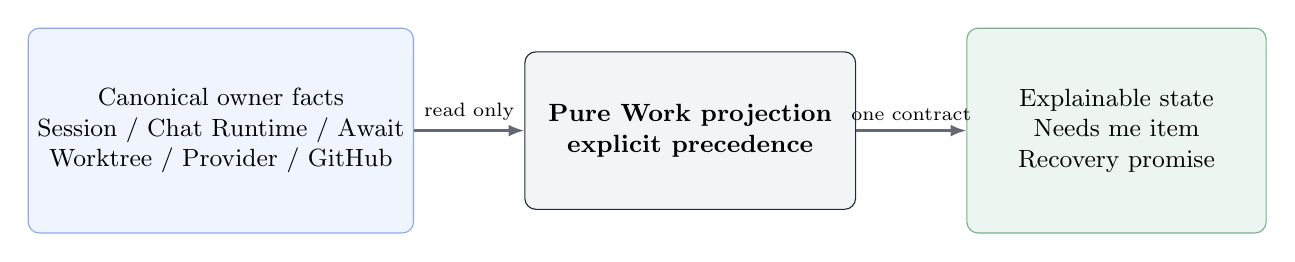
\begin{tikzpicture}[
  node distance=14mm,
  owner/.style={draw=cradleblue!55,fill=cradleblue!7,rounded corners,minimum width=40mm,minimum height=26mm,align=center,font=\small},
  core/.style={draw=cradleink,fill=cradlegray,rounded corners,minimum width=42mm,minimum height=20mm,align=center,font=\small\bfseries},
  output/.style={draw=cradlegreen!60,fill=cradlegreen!8,rounded corners,minimum width=38mm,minimum height=26mm,align=center,font=\small},
  arrow/.style={-{Latex[length=2mm]},thick,draw=cradleink!70}
]
\node[owner] (facts) {Canonical owner facts\\Session / Chat Runtime / Await\\Worktree / Provider / GitHub};
\node[core,right=of facts] (projection) {Pure Work projection\\explicit precedence};
\node[output,right=of projection] (outputs) {Explainable state\\Needs me item\\Recovery promise};
\draw[arrow] (facts) -- node[above,font=\scriptsize]{read only} (projection);
\draw[arrow] (projection) -- node[above,font=\scriptsize]{one contract} (outputs);
\end{tikzpicture}
\caption{No fact is copied from its owning module; Work produces a read model.}
\end{figure}

The API returns state and state-change time together with an explanation.  The
explanation contains the trigger, evidence, authority, responsible party, and
next action.  Recovery evidence and heartbeat time are separate fields.  Fresh
redetection rereads canonical facts and is idempotent.

\subsection{State selection}

The first matching row in Table~\ref{tab:precedence} wins.  This makes conflict
resolution reviewable and unit-testable rather than dependent on UI timing.

\begin{table}[ht]
\centering
\small
\begin{tabularx}{\textwidth}{@{}r l l X@{}}
\toprule
Priority & State & Authority & Winning fact / required action \\
\midrule
1 & archived & user action & Work or primary Session archived; restore only to continue. \\
2 & done / cancelled & structured owner & GitHub reports merged / closed without merge. \\
3 & failed & runtime or owner & Session error or unhealthy isolation; inspect and repair. \\
4 & awaiting human & runtime integration & Structured input or tool approval is pending. \\
5 & awaiting dependency & structured owner & A Session Await is pending. \\
6 & running & runtime integration & Active run or streaming Session. \\
7 & merging & structured owner & Open non-draft pull request needs merge decision. \\
8 & ready for review & owner/runtime & Draft PR or handoff newer than last submit. \\
9 & verifying & derived & Submit exists but current PR fact is unavailable. \\
10 & unknown & derived & No supported fact justifies a stronger claim; redetect or inspect. \\
\bottomrule
\end{tabularx}
\caption{Implemented state precedence. ``Unknown'' is a diagnostic result, not
a hidden success state.}
\label{tab:precedence}
\end{table}

The roadmap vocabulary also reserves draft, queued, and preparing.  They remain
stable API values but are intentionally not synthesized from weak signals in
this slice.  A future persisted Work event stream may make those transitions
observable without guessing.

\subsection{Attention and recovery}

Actionable states map to only four inbox categories: approve/answer, handle
failure, review, and merge/archive.  Items include Work identity, runtime,
provider/agent identifiers, risk, wait duration, reason, authority, recovery,
and next action.  Ordering is risk descending, waiting time descending, then
title.  The existing \code{/awaits} route is preserved as a compatibility
surface while its user-facing content becomes \emph{Needs me}.

Recovery is the strongest currently supportable promise rather than four
independent badges:

\begin{figure}[ht]
\centering
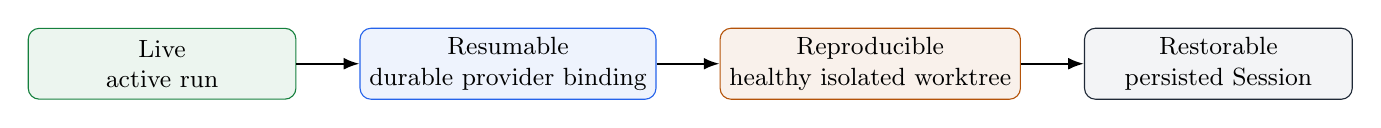
\begin{tikzpicture}[
  level/.style={draw,rounded corners,minimum width=34mm,minimum height=9mm,align=center,font=\small},
  arrow/.style={-{Latex[length=2mm]},thick}
]
\node[level,draw=cradlegreen,fill=cradlegreen!8] (live) {Live\\active run};
\node[level,draw=cradleblue,fill=cradleblue!8,right=8mm of live] (resume) {Resumable\\durable provider binding};
\node[level,draw=cradleamber,fill=cradleamber!8,right=8mm of resume] (reproduce) {Reproducible\\healthy isolated worktree};
\node[level,draw=cradleink,fill=cradlegray,right=8mm of reproduce] (restore) {Restorable\\persisted Session};
\draw[arrow] (live) -- (resume);
\draw[arrow] (resume) -- (reproduce);
\draw[arrow] (reproduce) -- (restore);
\end{tikzpicture}
\caption{Selection order for the strongest immediately useful recovery fact.
Unknown is returned when none is available.}
\end{figure}

\section{Implementation surface}

The change adds a Drizzle migration for newline-independent JSON acceptance
criteria, a pure server projection and tests, aggregate/API routes for attention
and redetection, generated TypeScript clients, localized Work badges, the Needs
me view, New Work acceptance-criteria capture, and a deeper Work Cucumber
journey.  Principal source locations are:

\begin{itemize}
  \item \code{apps/server/src/modules/work/projection.ts} and
        \code{projection.test.ts};
  \item \code{apps/server/src/modules/work/service.ts}, \code{model.ts}, and
        \code{index.ts};
  \item \code{apps/web/src/features/work/work-attention*.tsx} and
        \code{work-header-chrome*.tsx};
  \item \code{apps/web/src/features/new-work/new-work-acceptance-criteria-view.tsx};
  \item \code{packages/db/drizzle/0056\_lame\_black\_bolt.sql}; and
  \item \code{e2e/src/features/work.feature} plus its page object and steps.
\end{itemize}

\section{Evaluation method}

\subsection{Evidence hierarchy}

The evaluation uses four layers.  A higher layer does not replace the lower
one; it checks a different failure class.

\begin{enumerate}
  \item \textbf{Pure policy tests}: exhaustive table cases for state precedence
        and recovery selection.
  \item \textbf{Aggregate and UI tests}: persistence round-trip, generated type
        contract, badge behavior, empty/error states, direct action, and
        duration formatting.
  \item \textbf{Static and build checks}: TypeScript, module boundaries, API
        generation, and production Vite bundling.
  \item \textbf{Real-browser dogfood}: Cucumber launches an isolated server,
        production web preview, Playwright Chromium, real managed Git worktree,
        real Claude Agent adapter, and the repository model API simulator.
\end{enumerate}

The dogfood scenario enters an objective and explicit acceptance criterion,
starts Work, lets the runtime perform a tool loop that writes a real file,
waits for idle, and then independently verifies the database-backed API,
worktree path and contents, status explanation, recovery promise, rendered
badges, direct Needs me navigation, and simulator exhaustion.

\subsection{Measured results}

\begin{table}[ht]
\centering
\small
\begin{tabularx}{\textwidth}{@{}X l X@{}}
\toprule
Check & Result & Evidence \\
\midrule
Projection + Work service focused tests & \pass & 44 Vitest assertions across 2 files. \\
Work/New Work web focused tests & \pass & 40 Vitest assertions across 14 files. \\
Server and web TypeScript & \pass & Both application typechecks exited 0. \\
Server module boundaries & \pass & Direct boundary checker exited 0; largest existing SCC reported. \\
Production web bundle & \pass & Vite production build completed during browser dogfood. \\
Target Work dogfood & \pass & 1 scenario, 16/16 steps; 69.121 seconds wall time. \\
Full active P0/P1 E2E suite & \pending & Two monolithic runs were environment-terminated; a known cross-scenario Read race reproduced, while the same scenario passed 12/12 in isolation. Native Codex startup was blocked by outer network approval. \\
Full server test suite & \pending & 1711 passed, 2 skipped, 9 failed from existing environment assumptions (root Claude bypass, missing Go/relayd, default Documents path, and Codex assertions). \\
\bottomrule
\end{tabularx}
\caption{Validation evidence captured on the implementation branch.}
\label{tab:results}
\end{table}

Two environment failures occurred before the successful target run: the
Playwright CDN returned a truncated zero-byte archive, and its private ffmpeg
binary was absent.  The harness was kept intact.  Chromium 149 was obtained
through the allowed npm registry, the system ffmpeg 6.1.1 was supplied at the
Playwright runtime path, and a standalone page launch first proved the browser
was real.  A separate first target failure exposed a page-object lifetime bug
in the new E2E test; the Work id is now stored in scenario state.  This is useful
dogfood evidence because it prevented a false pass while leaving product state
correct.  The full active suite was then attempted twice with the synced Codex
app-server.  Both runs advanced through the non-Codex journeys before the outer
sandbox cancelled a network approval at native Codex startup.  The existing
Claude Read journey also showed a cross-scenario race (no activity feed after
the preceding reset); the identical scenario passed all 12 steps when isolated.
Accordingly, this report marks the monolithic suite inconclusive rather than
passed or product-failed.

\section{Assessment against the 30-day thresholds}

Table~\ref{tab:metrics} separates verified mechanism from production metrics.
One deterministic dogfood sample cannot establish a fleet-level percentile or
error rate.

\begin{table}[ht]
\centering
\small
\begin{tabularx}{\textwidth}{@{}X l X@{}}
\toprule
Roadmap threshold & Status & Interpretation \\
\midrule
$\geq95\%$ active Work automatically classifiable & \gate & Contract and precedence are implemented; collect at least one week of real Work labels before claiming the rate. \\
$\geq90\%$ Needs me direct correct action & \gate & Direct navigation passed dogfood; correctness rate requires human annotation across real items. \\
$<5\%$ false interruption from misclassification & \gate & Unknown and evidence visibility reduce silent error; production confusion matrix is still required. \\
$\geq99\%$ restart association integrity & \gate & Session/Work/base facts persisted in the browser scenario; restart cohort measurement is not yet instrumented. \\
Create-to-first-run P50 $<45$s, P95 $<120$s & \gate & This study measures end-to-end scenario time, not a statistically valid startup latency distribution. \\
\bottomrule
\end{tabularx}
\caption{Honest threshold assessment: feature verification is not a substitute
for production telemetry.}
\label{tab:metrics}
\end{table}

\section{Validity limits and risks}

\begin{itemize}
  \item \textbf{External validity}: simulator wire behavior is deterministic;
        provider outages and long-running terminal edge cases require live
        dogfood labels.
  \item \textbf{State coverage}: draft, queued, and preparing need structured
        lifecycle events before they can be truthfully emitted.
  \item \textbf{Timestamp precision}: existing owner rows supply seconds-level
        timestamps.  Await start time is not yet exposed by the summary owner,
        so that state conservatively falls back to Work update time.
  \item \textbf{GitHub semantics}: an open, non-draft PR is labeled ``Ready to
        merge'' in the UI while the API state remains \code{merging}; the report
        treats it as a user merge decision, not proof that a merge command is
        currently running.
  \item \textbf{Scale}: attention currently performs live PR reads through the
        existing Work list behavior.  Larger installations should add event
        caching or batching without weakening freshness explanations.
\end{itemize}

\section{Next-phase gates}

\begin{figure}[ht]
\centering
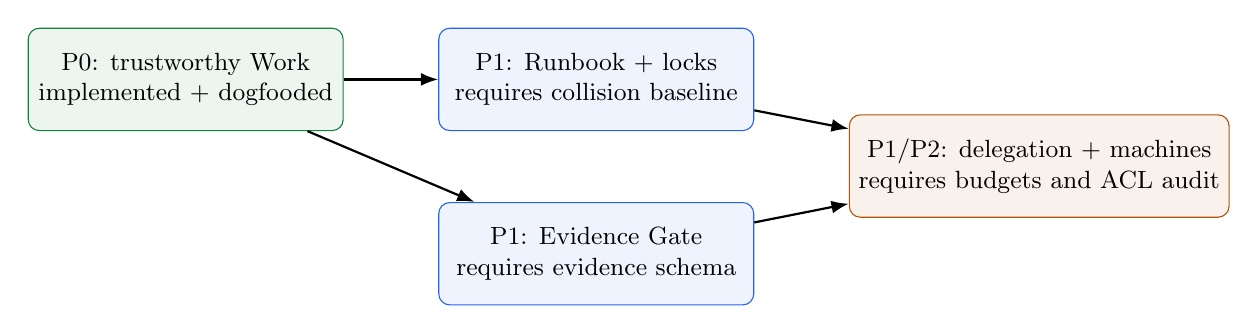
\begin{tikzpicture}[
  phase/.style={draw,rounded corners,minimum width=40mm,minimum height=13mm,align=center,font=\small},
  arrow/.style={-{Latex[length=2.2mm]},thick}
]
\node[phase,draw=cradlegreen,fill=cradlegreen!8] (p0) {P0: trustworthy Work\\implemented + dogfooded};
\node[phase,draw=cradleblue,fill=cradleblue!8,right=12mm of p0] (p1a) {P1: Runbook + locks\\requires collision baseline};
\node[phase,draw=cradleblue,fill=cradleblue!8,below=9mm of p1a] (p1b) {P1: Evidence Gate\\requires evidence schema};
\node[phase,draw=cradleamber,fill=cradleamber!8,right=12mm of p1a,yshift=-11mm] (p2) {P1/P2: delegation + machines\\requires budgets and ACL audit};
\draw[arrow] (p0) -- (p1a);
\draw[arrow] (p0) -- (p1b);
\draw[arrow] (p1a) -- (p2);
\draw[arrow] (p1b) -- (p2);
\end{tikzpicture}
\caption{Recommended release gates preserve the roadmap's dependency order.}
\end{figure}

Before the next implementation round, dogfood should record real Work links,
elapsed time, failure class, and one user quote for the five roadmap questions.
P1 should begin only after (a) state confusion and Needs me action correctness
have labeled baselines, (b) the most common port/shared-resource collisions are
known, and (c) the smallest review evidence schema is agreed.  Delegation and
machine sharing should remain off until budget stop/recovery and authorization
auditing have executable acceptance tests.

\section{Conclusion}

The implementation demonstrates that Cradle can become a local-first delivery
control plane by composing facts it already owns.  Work now has a single,
explainable delivery projection; Needs me supplies a cross-Work attention path;
and recovery language is bounded by observable durability.  The successful
real-browser journey establishes functional feasibility and catches integration
errors that unit tests could not.  It does not, by itself, establish the
roadmap's production percentages.  Those remain explicit measurement gates,
which is the correct boundary between a successful P0 engineering slice and a
90-day product outcome claim.

\end{document}
